\chapter{Estrutura e Materiais}

\section{Escopo}

\subsection{Local}

	O local escolhido para a casa sustentável foi o Jardim Botânico, 27a Região Administrativa do Distrito Federal. A escolha do Distrito Federal como local do projeto foi feita a partir de análises da média anual de radiação solar global diária do atlas solarmétrico do Brasil feito pela CEPEL, que indica que o estado do Distrito Federal se localiza em uma faixa de segundo maior índice de radiação solar dentro do Brasil, o que foi determinante para escolha do local, pois a energia proveniente do sol é uma das principais alternativas para a geração de energia da casa.
	
	Outro fator que foi levado em consideração para a escolha do DF, foi um ranking realizado pela ONU onde o estado está posicionado em um dos melhores lugares pelo IDHM, o que caracteriza melhor qualidade de vida no quesito educação, renda e expectativa de vida, se comparado ao restante dos estados brasileiros. Assim, delimitada a região do Distrito Federal, o Jardim Botânico foi escolhido por conter grandes lotes, com áreas que podem passar dos $1000\si{\meter}^{2}$\cite{2010Terracap} e áreas construidas acima de $250\si{\meter}^{2}$\cite{2014Codeplan}. O tamanho do lote foi priorizado na escolha da localidade pois grandes áreas são necessárias para a implantação de tecnologias sustentáveis, como painéis solares e turbinas eólicas.
	
	Outro fator que foi determinante para a escolha da localização foi a renda domiciliar da região, que no Jardim Botânico no ano de 2013 teve média de 18,51 salários mínimos\cite{2013SeplanCodeplan}. O projeto de uma casa sustentável engloba o uso de tecnologias inovadoras e de alto custo, assim, o projeto visa atender famílias de alta renda.
	
\subsection{Número de Pessoas}

	A partir da análise de dados do IBGE\cite{2010IBGE} verificamos que a média do número de componentes das famílias brasileiras varia entre 3,2 a 3,6 pessoas por residência. Considerando que na definição do projeto pretendemos buscar que a casa seja versátil, podendo suportar visitas e um eventual aumento da família, arrendondamos os números do IBGE\cite{2010IBGE} para mais, definindo para 4 o número de componentes da família. 

\section{Definições}

\subsection{Construção Sustentável}
	
	A construção sustentável é um processo produtivo que tende a realizar, no entorno, alteração conscientes, de forma a suprir as necessidades do uso do homem e de edificação, preservando os recursos naturais e o meio ambiente, garantindo para as gerações atuais e futuras uma qualidade de vida\cite{1992Baroni}. Para uma construção sustentável é necessário analisar o planejamento sustentável da obra, o aproveitamento passivo dos recursos naturais, a eficiência energética, a gestão e economia de água, a qualidade do ar e do ambiente interior, uso racional de materiais e o uso de produtos e tecnologias amigáveis ambientalmente\cite{2012Araujo}.






















































%%%%%%%%%%%%%%%%%%%%%%%%%%%%%%%%%%%%%%%%%%%%%%%%%%%%%%%%%%%%%%%%%%%%%%%%%%%%%%%%%%%%%%%%%%%%%%%%%%%%%%%%%%%%%%%%%%%%%%%%%%%%%%%%%%%%%%%%%%%%%%%%%%%%%%%%%%%%%%%%5
\section{Local}
	O local escolhido para a casa sustentável foi o Jardim Botânico, 27$^a$ Região Administrativa do Distrito Federal.

	A escolha do Distrito Federal como local do projeto foi feita a partir de análises da média anual de radiação solar global diária do atlas solarmétrico do Brasil feito pela CEPEL, que indica que o estado do Distrito Federal se localiza em uma faixa de segundo maior índice de radiação solar dentro do Brasil, o que foi determinante para escolha do local, pois a energia proveniente do sol é uma das principais alternativas para a geração de energia da casa.

	Outro fator que foi levado em consideração para a escolha do DF, foi um ranking realizado pela ONU onde o estado está posicionado em um dos melhores lugares pelo IDHM, o que caracteriza melhor qualidade de vida no quesito educação, renda e expectativa de vida, se comparado ao restante dos estados brasileiros.

	Assim, delimitada a região do Distrito Federal, o Jardim Botânico foi escolhido por conter grandes lotes, com áreas que podem passar dos 1000$\textup{m}^{2}$%\cite{5298d86a7fd17}
 e áreas construidas acima de 250$\textup{m}^{2}$%\cite{PDAD}
. O tamanho do lote foi priorizado na escolha da localidade pois grandes áreas são necessárias para a implantação de tecnologias sustentáveis, como painéis solares e turbinas eólicas.

	Outro fator que foi determinante para a escolha da localização foi a renda domiciliar da região, que no Jardim Botânico no ano de 2013 teve média de 18,51 salários mínimos%\cite{pesquisa_socioeconomica}
. O projeto de uma casa sustentável engloba o uso de tecnologias inovadoras e de alto custo, assim, o projeto visa atender famílias de alta renda.

\section{Construção sustentável}

	A construção sustentável é um processo produtivo que tende a realizar, no entorno, alteração conscientes, de forma a suprir as necessidades do uso do homem e de edificação, preservando os recursos naturais e o meio ambiente, garantindo para as gerações atuais e futuras uma qualidade de vida\cite{Baroni1992}. Para uma construção sustentável é necessário analisar o planejamento sustentável da obra, o aproveitamento passivo dos recursos naturais, a eficiência energética, a gestão e economia de água, a qualidade do ar e do ambiente interior, uso racional de materiais e o uso de produtos e tecnologias amigáveis ambientalmente\cite{Araujo2012}.

\section{Materiais}

	Há dois tipos de materiais, além do convencional, que podem ser usados na construção de uma casa sustentável:

\begin{itemize}

	\item \textbf{Materiais Sustentáveis} – Referem-se a materiais que abordam benefícios para toda construção, entorno e meio ambiente, sem serem necessariamente naturais.

	\item \textbf{Materiais Ecológicos} – Referem-se a materiais produzidos com matérias-primas naturais renováveis ou não-renováveis. Materiais extração local ou próximo dos locais de uso e materiais com pouco consumo de energia e água para sua obtenção, transformação e beneficiamento.

\end{itemize}

\subsection{Escolha dos Materiais}

	Na escolha dos materiais devem ser consideradas a origem da matéria-prima, extração, processamento, gastos com energia para transformação, emissão de poluentes, biocompatibilidade, durabilidade, qualidade, entre outros que permitam classifica-los como sustentáveis ou ecológicos e elevar o padrão da obra no quesito de melhoria da qualidade de vida de seus habitantes e do próprio entorno. Essas características analisadas, devem estar de acordo com a geografia, tipologia, ecossistema, condições climáticas, resistência, responsabilidade social do ambiente onde será construído.

\subsection{Possíveis Materiais}

\subsubsection{Pisos – Ambiente Interno (Seco)}

	Caracteriza-se ambiente seco lugares onde não entram em contato com água frequentemente, como a sala, os quartos, escritórios e etc.\\

\textbf{Piso de bambu}

	Em comparação com outras madeiras, o bambu tem crescimento muito rápido, com alta produtividade por hectare, além de ser altamente renovável e sustentável. O piso de bambu é mais forte, mais estável e mais durável do que a maioria dos pisos de outros tipos de madeira. Possui maior estabilidade dimensional e, portanto, menos expansão e contração do que pisos de madeiras tradicionais. A opção do piso de bambu traz um design à casa, o material está na moda no mercado e sua variedade de tonalidades que o próprio bambu tem aumenta o conforto do morador.

\begin{itemize}
\item \textbf{Vantagens do bambu}
\begin{itemize}
	\item O bambu é relativamente forte e rígido
	\item O bambu pode ser cortado com ferramentas simples.
	\item A superfície do bambu é dura e limpa
	\item O bambu pode ser cultivado em pequena escala
	\item O retorno do capital é mais rápido do que se fosse usada madeira.
	\item As estruturas de bambu são flexíveis durante tormentas e terremotos
	\item O bambu pode ser usado com sucesso para reforçar um terreno deficiente, como por exemplo evitar desabamentos de terra ou para reforçar um caminho.
\end{itemize}

\item \textbf{Desvantagens do bambu}
\begin{itemize}
	\item O bambu tem uma durabilidade natural baixa e necessita de tratamento
	\item O fogo representa um grande risco.
	\item Os talos do bambu não são totalmente retos, são estreitos. As emendas estão a distâncias diferentes e podem ser importunas quando se trabalha o material.
	\item A normalização é praticamente impossível devido à variação dos tamanhos.
\end{itemize}

\item \textbf{Fábricas no Brasil}

\textbf{Ditzel} - Fabricante, Prudentopolis – PR\\
\textbf{Lisonda} - Fabricante, Taboão da Serra - SP\\
\textbf{Alphenas Design} - Fabricante, Taboão da Serra - SP
\end{itemize}

\subsubsection{Piso – Ambiente externo (Molhado)}
	Caracteriza-se ambiente molhado lugares que entram em contato com água frequentemente, como banheiros, área de serviços, entre outros.

\begin{itemize}

\item \textbf{Piso Cerâmico}

	No processo produtivo da cerâmica há reaproveitamento de sobras reduzindo os impactos ambientais, como o uso da água e argila por exemplo.

\item \textbf{Vantagens:}
\begin{itemize}
\item \textbf{Durabilidade}\\O piso cerâmico é muito mais durável que outro tipo de pisos. É também muito resistente à água e bactérias, sendo por isso uma boa opção para quem sofra de problemas respiratórios ou alergias. Devidamente instalado, o piso de cerâmica por durar por 20 anos ou até mais.

\item \textbf{Variedade de modelos}\\O piso cerâmico pode ser encontrado em diversas cores, desde as mais vibrantes aos tons mais sóbrios. Alguns modelos de pisos cerâmicos apresentam também textura ou imitam, inclusive, pisos considerados mais nobres, como madeira ou mármore. Como este tipo de piso é vendido à peça, é possível criar padrões elegantes ou mais originais, dependendo da forma como são dispostas as telhas no chão.

\item \textbf{Isolamento}\\Em climas mais secos e quentes, o piso cerâmico ajuda a manter a temperatura ambiente mais fresca.

\item \textbf{Preço}\\Uma vez que o piso cerâmico é mais durável, o seu valor é considerado um bom investimento face a outros tipos de piso mais caros.

\item \textbf{Instalação}\\A própria de instalação também fica mais econômica, sendo também muito simples de ser feita.

\item \textbf{Fácil manutenção}\\Este tipo de piso tem uma manutenção muito simples, para além de ser muito fácil de limpar. Para o manter bonito e nas melhores condições basta simplesmente varrer o chão, limpando de seguida com um esfregão úmido e um pouco de detergente doméstico suave.

\end{itemize}
\item \textbf{Desvantagens:}

\begin{itemize}
\item \textbf{Isolamento}\\Embora o piso cerâmico seja ideal para climas mais quentes, visto dar frescura ao ambiente, em climas mais frios pode tornar-se demasiado gelado quando em contato com os pés.

\item \textbf{Escorregadio}\\Quando molhado este tipo de piso pode levar a quedas e fraturas, uma vez que se torna muito escorregadio. É por isso aconselhável que esteja bem seco antes de alguém o pisar.

\item \textbf{Delicado}\\Durante a sua instalação o piso cerâmico pode ser muito delicado, podendo inclusive partir-se com alguma facilidade, quando não são tidos todos os cuidados necessários para a sua correta colocação no chão.

\item \textbf{Superfície dura}\\Ao contrário de outro tipo de pisos, como o piso em carpete, o piso cerâmico apresenta uma superfície muito dura. Em casas com crianças pequenas é aconselhável que se utilize tapetes nas zonas de maior passagem e brincadeiras, para que exista uma superfície mais fofa no caso de quedas.

\end{itemize}


\item \textbf{Fábricas no Brasil}

\textbf{Itagres} - São Cristóvão - Tubarão – SC\\
\textbf{Portobello S.A.} - Tijucas - SC – Brasil

\end{itemize}

\subsubsection{Paredes}
\begin{itemize}

\item \textbf{Tijolo Ecológico (solo-cimento)}

	Solo-cimento é o material obtido pela mistura de solo, cimento e água. O tijolo deste material é feito pela prensa, manual ou automatizada, dessa mistura. Após a prensa ele passa pela cura e secagem, não sendo necessária sua queima, que lançaria resíduos tóxicos no meio ambiente, enquanto no processo tradicional é feito a queima do tijolo logo após a saída da prensa. Portanto, no processo da queima no tijolo tradicional, há emissões de gases como CO2, SO2, CO, Gases Oxidantes, Óxidos Nitrogenados e Compostos de Chumbo, gases esses que contribuem para o aquecimento global e poluição do ar.\cite{Castro2011}

\item \textbf{Vantagens do tijolo ecológico:}

	Seu modelo de produção é por meio da prensa hidráulica ou eco manual, onde a pressão exercida é de 6 toneladas, tornando-o regular, com faces lisas e que proporcionam um encaixe perfeito, viabilizando assim uma maior precisão também no cálculo de tijolos necessários na obra;

	A utilização dos tijolos ecológicos evita a necessidade do uso de materiais como arame, madeira, pregos e folhas de parede pronta para a instalação da rede elétrica, hidráulica etc;

	Possui isolamento acústico e térmico, o que possibilita tanto o aquecimento como o resfriamento do ambiente de maneira natural;
Reduz a umidade nas paredes;

	Além de aumentar a resistência da estrutura, facilita toda a construção, uma vez que seu molde permite o encaixe fácil e rápido, sem a necessidade de utilização de gesso ou azulejos;

	Diferentemente dos tijolos tradicionais, os ecológicos necessitam de pequenas quantidades de cimento, dentre outros.

\item \textbf{Desvantagens do tijolo ecológico}

	Requer pedreiro qualificado, com conhecimento da técnica de aplicação;

	Apesar de funcionar perfeitamente bem em climas secos, os tijolos ecológicos, quando aplicados em locais de climas úmidos ou de maior exposição à umidade, ainda não é totalmente indicado.

\item \textbf{Fábricas no Brasil}

\textbf{PERMAQ - São Paulo} - SP – Brasil\\
\textbf{Monteiro Tijolos} - Salto – SP\\
\textbf{Sete Tijolos Ecológicos} - Campo Grande/MS

\end{itemize}

\subsubsection{Argamassa polimérica}

	Argamassas poliméricas são reconhecidas pelo forte apelo ecológico por não conterem em sua formulação os dois principais igredientes da argamassa cimentícia, ambos impactantes ao meio ambiente: Cimento Portland, que emitem CO$_2$ na atmosfera devido ao processo de descarbonificação e ao consumo de energia necessário para chegar a temperatura necessária. E areia de rios, com o uso da argamassa polimétrica, contribui-se para a diminuição da retirada desse material dos leitos dos rios. Sobretudo, as argamassas polimétricas reduzem o desperdício de materiais na construção e o consumo de energia elétrica necessário ao processo de mistura.\cite{Angulo2000}\cite{Portland1980}

	As vantagens estão associadas ao alto rendimento e o aumento da produtividade na fase de alvenaria. Além disso, como o produto não é a granel e possui maior rendimento, há melhor controle de estoque e redução do custo logístico. A utilização da argamassa polimérica, conforme informações dos fabricantes, garantem um aumento de produtividade de pelo menos 50\% e redução do custo total da alvenaria de pelo menos 40\%.

\begin{itemize}
\item \textbf{Fábricas no Brasil}

\textbf{Maxcon - Formiga} – MG\\
\textbf{Massa Dundun} - Pirituba – SP\\
\textbf{Masterfix} - Jacarezinho – PR
\end{itemize}

\subsubsection{Telhas}

\textbf{Telhas Ecológicas}

	São as telhas ecológicas, as quais são produzidas a partir de fibras naturais ou materiais reciclados. Seu uso ajuda a proteger o meio ambiente e traz vantagens para o consumidor. As telhas ecológicas podem ser utilizadas com as mesmas aplicações das telhas convencionais, pois as mesmas apresentam resultados melhores do que as telhas convencionais na caracterização mecânica, térmica e físico-química. Além do mais, as telhas ecológicas apresentam baixo custo de produção\\

\textbf{Vantagens}

\begin{itemize}
\item \textbf{Fácil manuseio e instalação}\\Seu estoque e transporte são fáceis (pois a telha é flexível) e reduzem o número de quebras / perda de material (é recomendado que seja utilizada mão-de-obra especializada);

\item \textbf{Economia de tempo e material}\\A maioria é mais leve que a telha
tradicional, reduzindo os custos da construção (a estrutura é mais leve e o
serviço é realizado rapidamente). É importante destacar que o planejamento é
essencial para a redução dos custos, ou seja, o desenvolvimento de um
bom projeto arquitetônico e estrutural é essencial, decidindo quais materiais
e acabamentos serão utilizados antes mesmo de iniciar a obra;

\item \textbf{É um material resistente}\\São resistentes e flexíveis, resistindo a chuvas de granizo;

\item \textbf{São anti-inflamáveis}\\A maioria não propaga chamas;

\item \textbf{São impermeáveis}\\Absorvem muito menos água do que as telhas convencionais e geralmente seu acabamento evita a proliferação de limo;

\item \textbf{Promovem o conforto térmico}\\Alguns tipos ajudam a criar um ambiente interno mais confortável (menos quente);

\item \textbf{Design}\\É possível encontrá-las em vários formatos e cores (inclusive pigmentada dos dois lados permitindo ser instalada sem forro). Além disso é possível pintá-las com tintas à base de água;

\item \textbf{São sustentáveis}\\Geralmente produzidas com fibras e resinas, materiais reciclados (como papel, caixa de leite longa vida) e não contém amianto (o qual é tóxico);

\item \textbf{Fábricas no Brasil}

\textbf{GLZ} – Telhas e Laminados Ecológicos -Santa Cruz do Sul – RS\\
\textbf{Eccoclean} Telhas Ecológicas - Saquarema – RJ\\
\textbf{ECO-LÓGICA} - Vicente Pires/DF

\end{itemize}

\section{Planta da Casa}

	A casa ecológica é uma nova tendência na área de construção, sendo caraterizada por possuir uma estrutura sustentável e não afetar o meio ambiente. Desta forma, a planta tem que ser planejada para que fatores ambientais como, vento, sol, frescor das plantas e outros, sejam melhores aproveitados.

	O formato da casa é um ponto importante a ser considerado no projeto, pois este determina como e quanto será utilizado de materiais. No caso de uma casa sustentável visamos o menor impacto ambiental possível e isso delimita as escolhas.

	Analisando as necessidades do nosso projeto e da família para qual ele será construído, determinou-se a nossa localidade no bairro Jardim Botânico, Df, e foi pautado a partir média das casas desse setor e das famílias que lá residem para determinar a área útil da casa e a formação da família.

	Fazendo uma média das 3 opções de planta, chegou-se a conclusão que a área da nossa planta será por volta de 226$\textup{m}^{2}$, pois o resto da área total do terreno precisa ser disponibilizada para suprir a nossa demanda energética. Acredita-se que 4 pessoas, ou até mais caso a família cresça, possam viver tranquilamente nesta área, com a distribuição de cômodos exemplificada na planta.

\begin{figure}[h]
\textbf{Opção 1}

	Garagem para dois carros, hall, sala de estar com lavabo, sala de jantar, cozinha americana com churrasqueira e acesso para varanda externa, piscina, área de serviços com despensa e lavanderia, suíte master com closet e duas demi-suites.

Área útil: 212$\textup{m}^{2}$, Área total: 460$\textup{m}^{2}$

  \begin{center}
	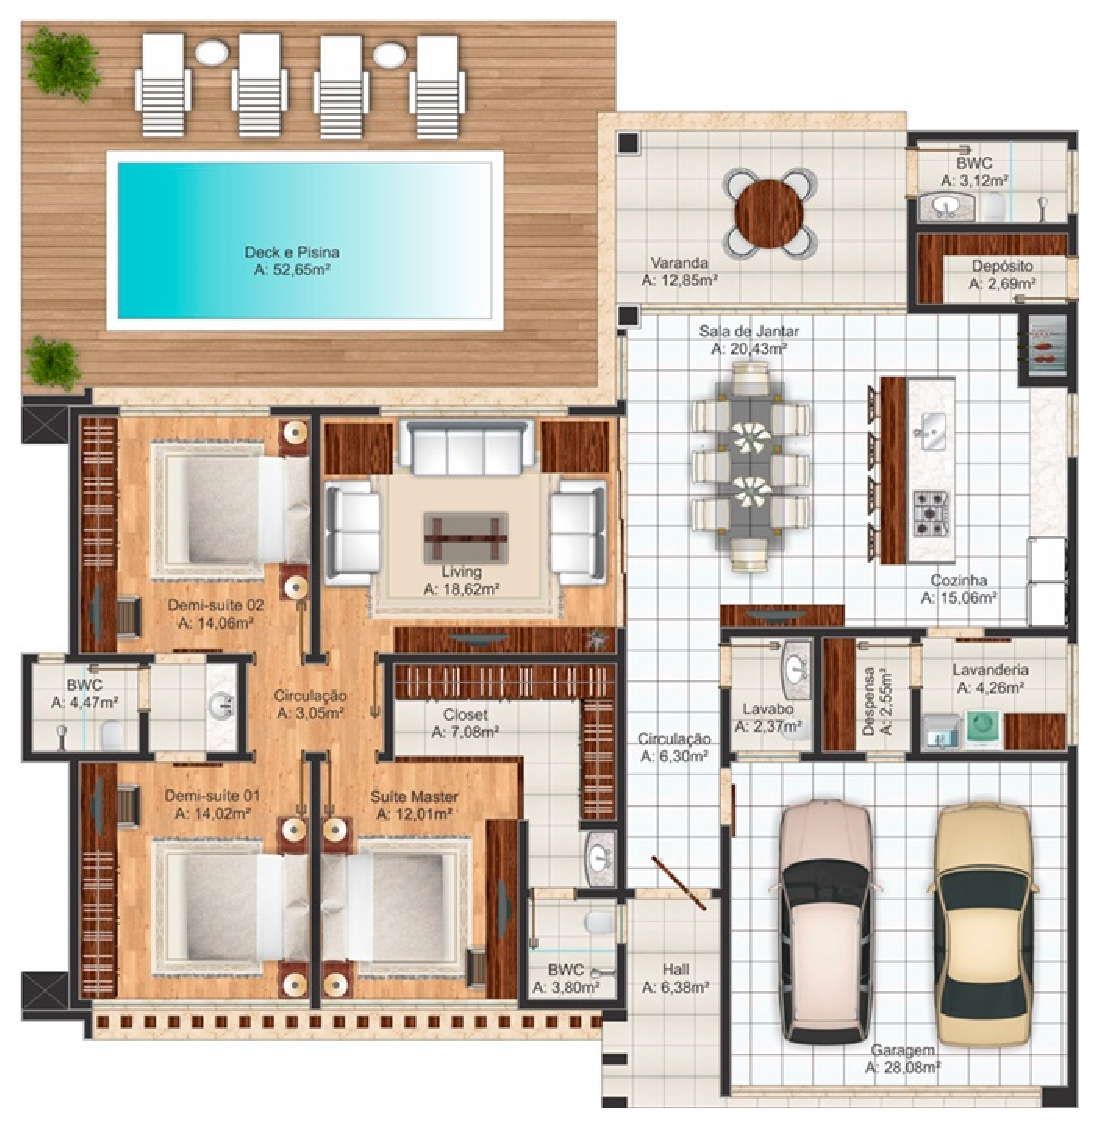
\includegraphics[keepaspectratio,scale=0.45]{figuras/planta1.eps}
	\caption{Planta 1}%\cite{planta1}}
  \end{center}
\end{figure}

\begin{figure}
\textbf{Opção 2}

	1 suite máster com closet e uma banheira com hidro, 2 demi-suítes, cozinha estilo americano, lavabo, sala de estar, sala de jantar, sala de jogos, lavanderia, varanda, área de lazer com piscina, churrasqueira e banheiro.

Área útil: 240$\textup{m}^{2}$, Área total: 524$\textup{m}^{2}$
\begin{center}
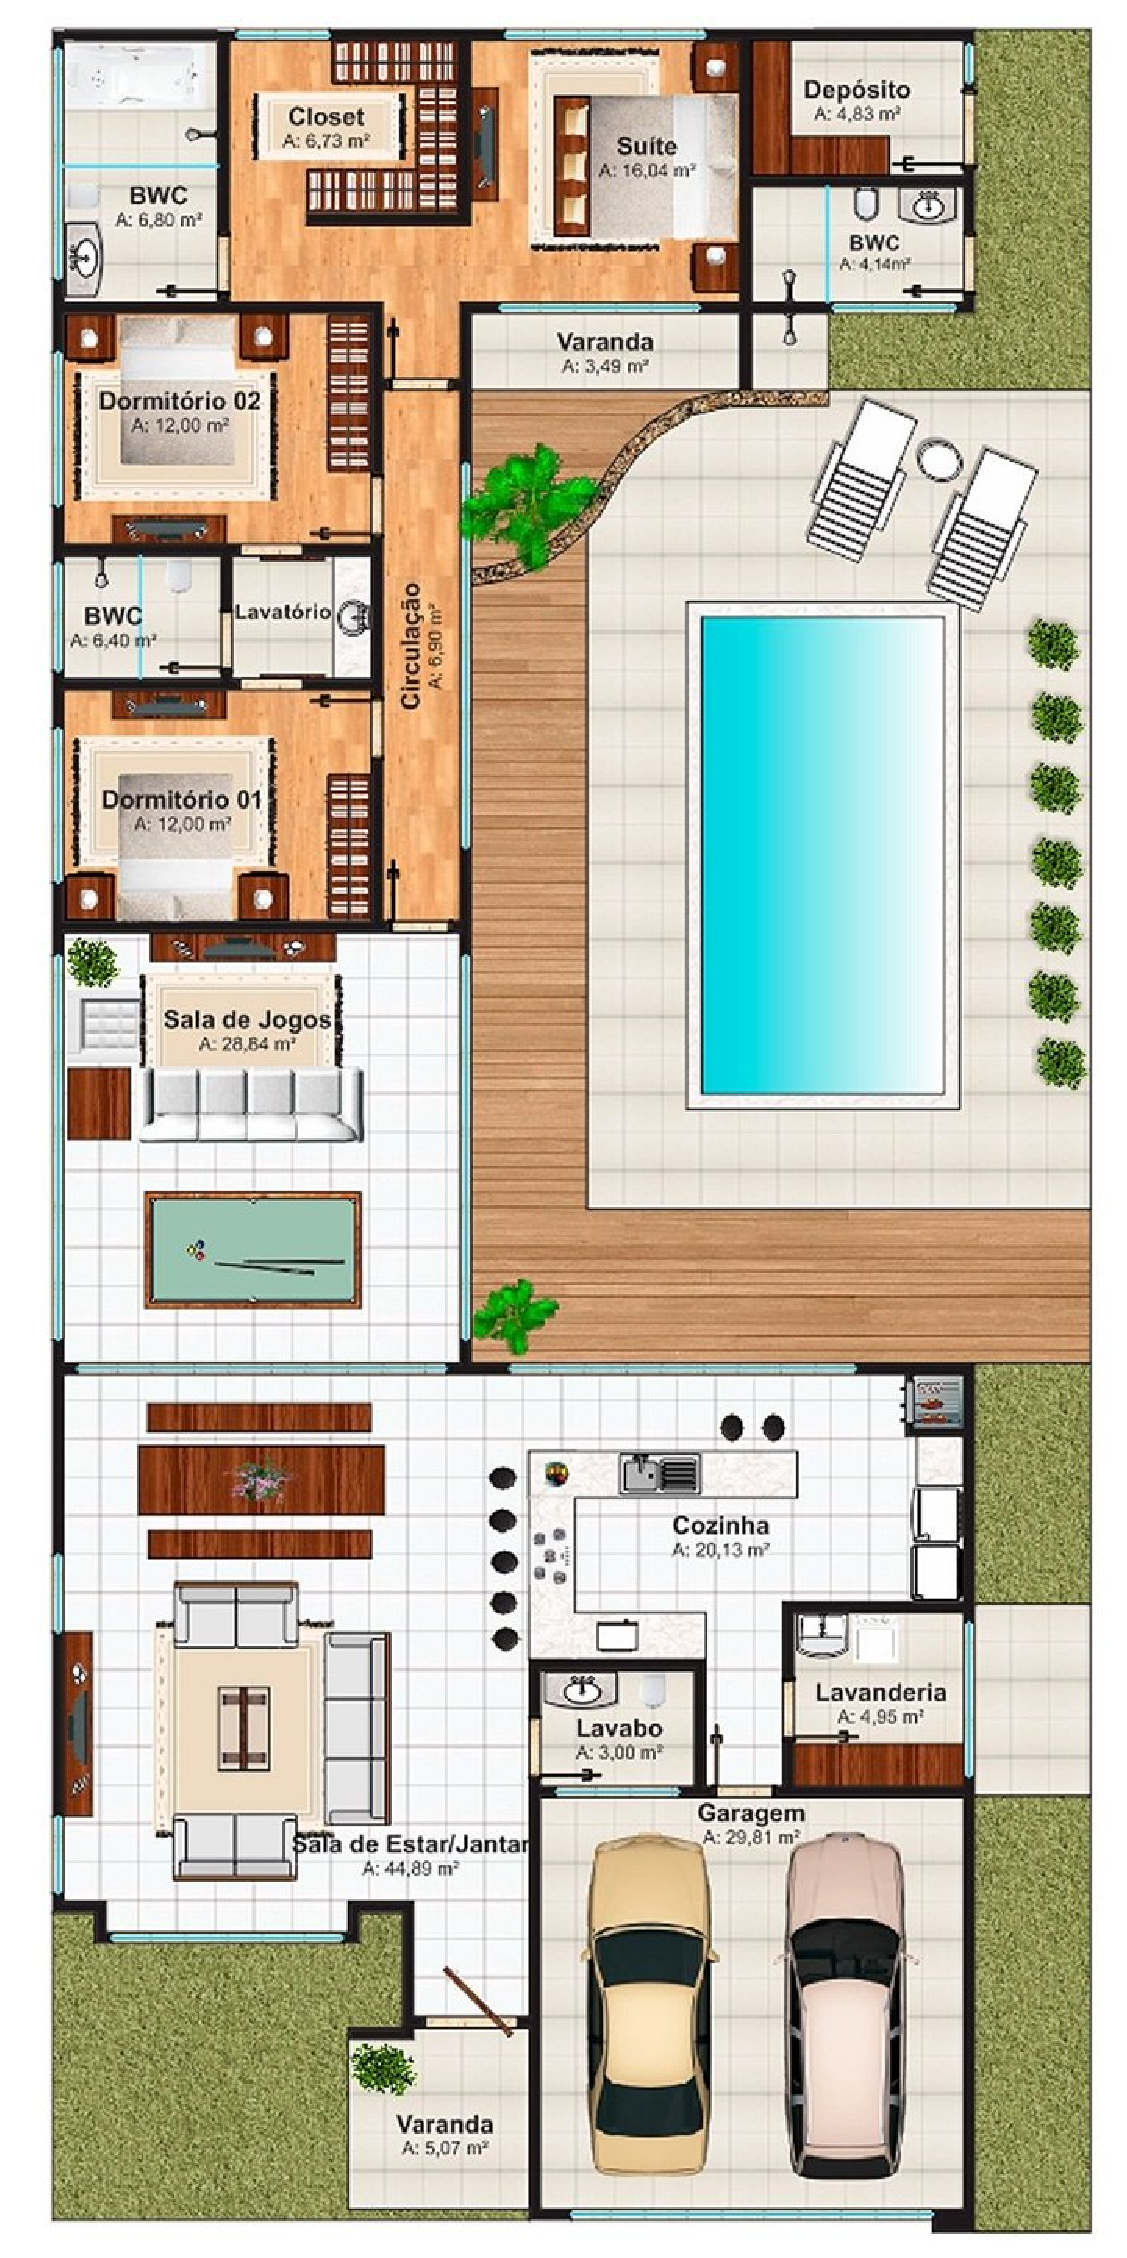
\includegraphics[keepaspectratio,scale=0.5]{figuras/planta2.eps}
\caption{Planta 2}%\cite{planta2}}
\end{center}

\end{figure}

\begin{figure}
\textbf{Opção 3}

	3 quartos com 2 suítes, 1 banheiro, 1 lavabo, cozinha, sala de estar, sala de jantar, 1 depósito, lavanderia, varanda, garagem para 2 carros e churrasqueira.

Área útil: 228$\textup{m}^{2}$, Área total: 486$\textup{m}^{2}$
\begin{center}
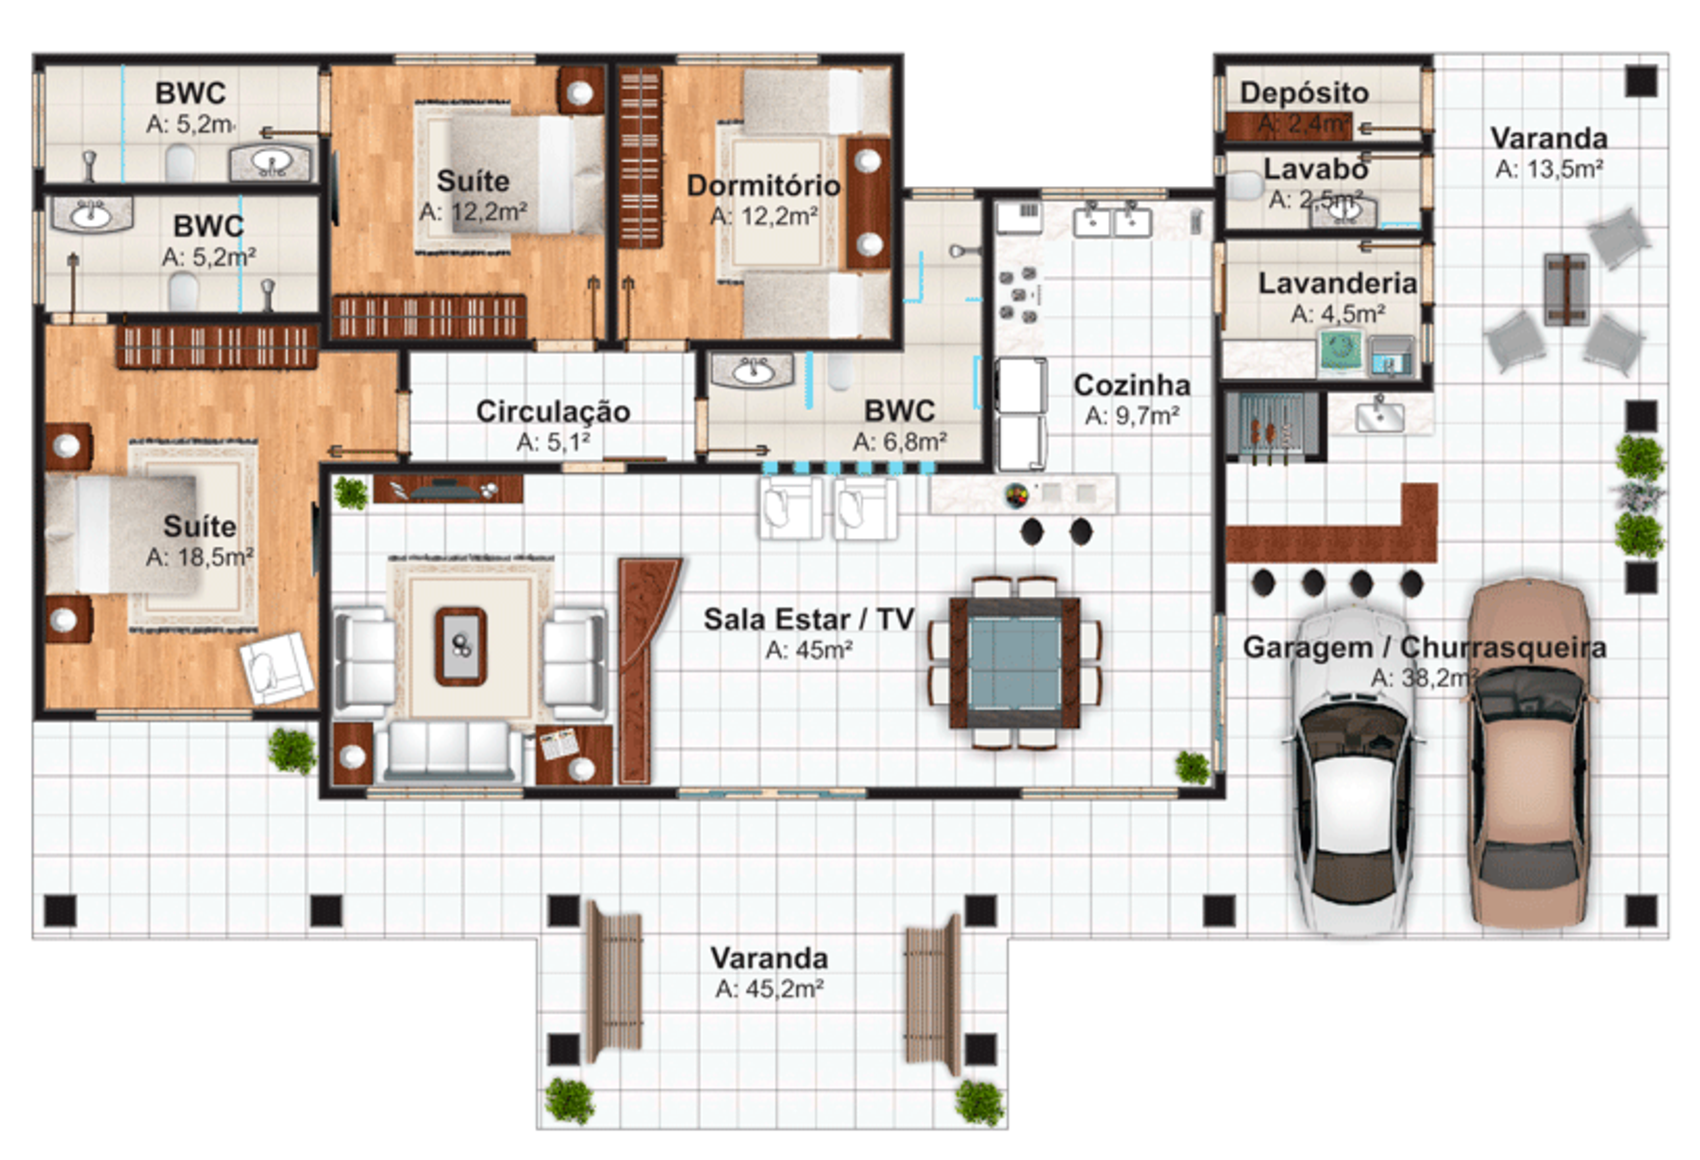
\includegraphics[keepaspectratio,scale=0.5]{figuras/planta3.eps}
\caption{Planta 3}%\cite{planta3}}
\end{center}
\end{figure}
